\chapter{Generators}
\textbf{Generator types used in power systems}
\begin{itemize}
    \item DC generator - usually separately excited machines in dedicated DC systems e.g. typically 5-\SI{600}{V_{DC}} output (still in service, rarely built)
    \item AC synchronous generator - by far the most common, can be single-phase or three-phase. Usually \SI{50}{\hertz} or \SI{60}{\hertz}; \SI{240}{\volt}-\SI{30}{\kilo\volt}; \si{\kilo\watt} to \si{\giga\watt}
    \item AC asynchronous generator - most common in renewable energy applications e.g. some wind-turbines. Usually three-phase, \SI{50}{\hertz} or \SI{60}{\hertz}; \SI{440}{\volt}-\SI{11}{\kilo\volt}; between 2-\SI{10}{\mega\watt}
\end{itemize}
\section{Synchronous machine}
Synchronous machines are the primary source of electrical energy generation (or conversion). They are used to convert the mechanical power output of steam-turbines, gas-turbines. reciprocating engines (prime movers), hydro turbines into electrical power. Synchronous machines can be extremely large with power ratings up to \SI{2}{\giga\watt} or very small at a few Watts. Known as synchronous machines because they operate at synchronous speeds (speed of rotor always determines supply frequency).
\subsection{Petrol/diesel generators}
\begin{itemize}
    \item Commonly used at low, medium and high powers (a few \si{\kilo\watt} to 10's \si{\mega\watt})
    \item Often direct connection between diesel and synchronous generator
    \item Efficiency typically 35\% at full load without waste heat recovery
    \item Efficiency typically 55\% at full load with waste heat recovery
    \item Commonly used at low powers: single-phase back-up power units
    \item Common use at medium powers: traction, ships, standby generators
    \item Common use at high powers in generating stations
\end{itemize}
\subsection{Gas turbine generators}
\begin{itemize}
    \item Commonly used at medium and high powers (\SI{1}{\mega\watt} to 10's \si{\mega\watt})
    \item Connected via gearbox at low powers and directly at high powers
    \item Efficiency typically 25\% at full load for simple cycle types
    \item Efficiency typically 55\% at full load in combined heat and power (CHP systems)
    \item Common use at medium powers: naval ships and standby generators
    \item Common use at high powers as CHP or CC in generating stations
\end{itemize}
\subsection{Steam turbine generators}
Steam turbine generators usually driven from coal-fired boilers or nuclear power. An example \SI{1.2}{\giga\watt} steam plant uses a hydrogen cooled generator.
\begin{itemize}
    \item Commonly used at medium and high powers (\SI{1}{\mega\watt} to several \si{\giga\watt})
    \item Connected via gearbox at low powers and directly at high powers
    \item Efficiency typically 60\% with sophisticated steam energy management system
    \item Common use at medium powers: ships using waste heat recovery
    \item Common use at high powers in the majority of power stations including nuclear
\end{itemize}
\subsection{Synchronous machine basics}
\begin{figure}[H]
    \centering
    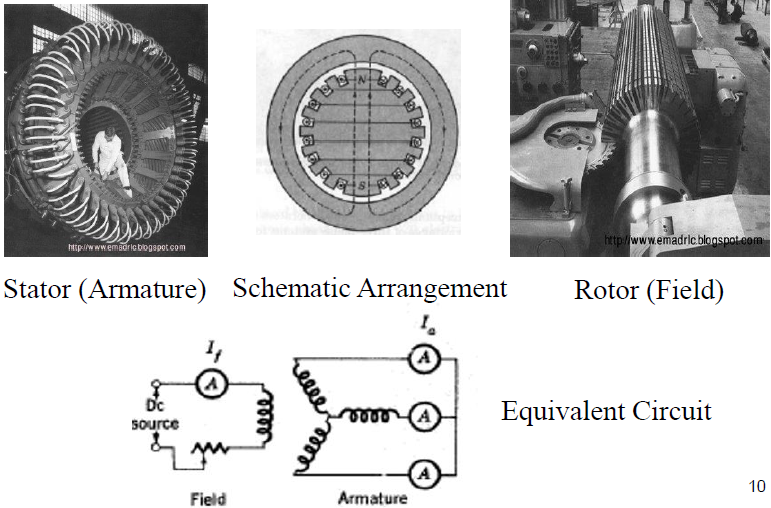
\includegraphics[width = 0.8\textwidth]{img/figure74.png}
    \caption{Synchronous machine basics.}
\end{figure}
\subsection{Concept of back emf and internal resistance}
\begin{figure}[H]
    \centering
    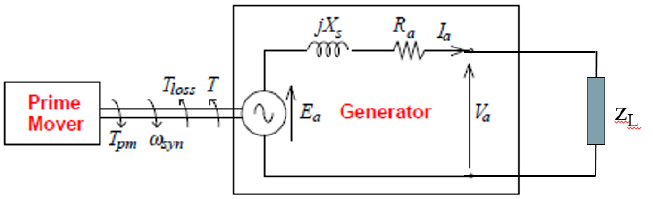
\includegraphics[width = 0.8\textwidth]{img/figure75.png}
    \caption{Generator diagram.}
\end{figure}
Back electro-motive force (emf = $Ea$) is always present in a power source as power supplies have internal resistance ($Ra$) and reactances $X$s which cause voltage drops internally and which increases as current flow increases ($Ia$).
\subsection{Phasor diagram representation}
\begin{figure}[H]
    \centering
    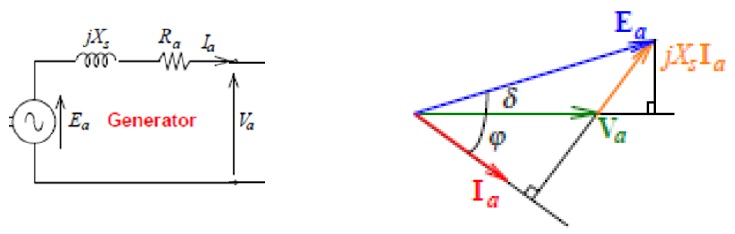
\includegraphics[width = 0.8\textwidth]{img/figure76.png}
    \caption{Phasor diagram.}
\end{figure}
The voltage drops can be represented in a phasor diagram. There are two important angles in this diagram known as $\phi$ and $\delta$.
\begin{itemize}
    \item $\phi$ is the phase angle (cosine of this angle is the power factor)
    \item $\delta$ is the load angle
\end{itemize}
Which conditions must exist for $Ea = Va$?
\begin{figure}[H]
    \centering
    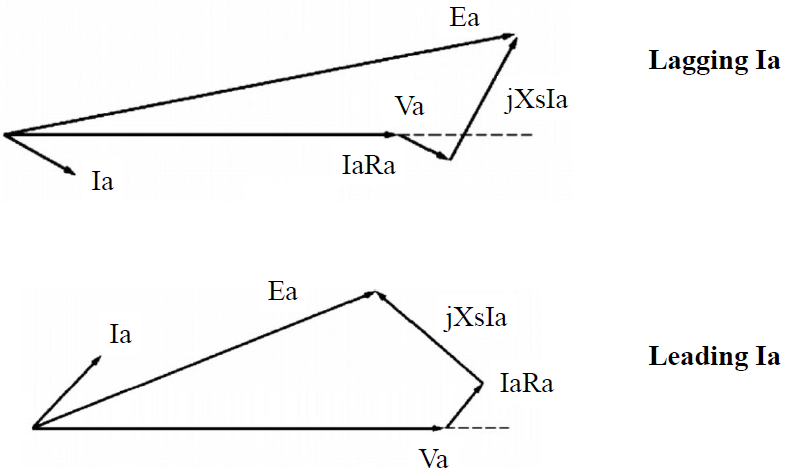
\includegraphics[width = 0.8\textwidth]{img/figure77.png}
    \caption{Current magnitude and phase effects on $Va$.}
\end{figure}
\subsection{The speed of rotation of synchronous generators}
The electrical frequency is synchronised to the rotor speed. Recall that the magnetic field created by a 3-phase 4-pole machines moves \SI{180}{\degree} while the stator currents vary \SI{360}{\degree}.
\begin{gather}
    f_e(\si{\hertz}) = \frac{n_m\left(\si{r\per min}\right)P\#}{120}
\end{gather}
Therefore, a 2-pole generator must turn at \SI{3600}{r\per min} to produce a \SI{60}{\hertz} voltage while a 4-pole must turn at \SI{1500}{r\per min} to produce a \SI{50}{\hertz} power.
\subsection{Frequency and voltage control}
Governor control: frequency is controlled by the speed of rotation and the number of poles/ As the latter is fixed (a construction constraint) it is the speed of rotation that is important.

Automatic voltage regular control: voltage is controlled by the magnetic flux in the air gap in a fixed speed machine. This is essentially controlled by the field current within magnetic saturation limits.
\subsection{Control of generators}
\begin{figure}[H]
    \centering
    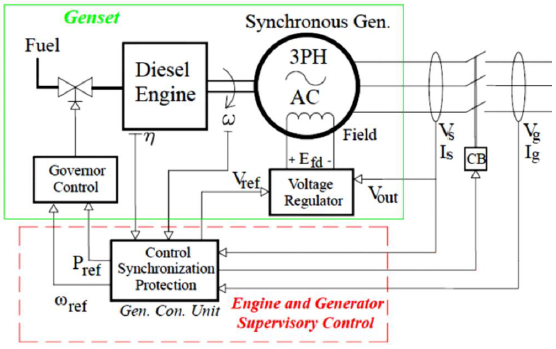
\includegraphics[width = 0.8\textwidth]{img/figure78.png}
    \caption{Control of generators.}
\end{figure}
The diesel-generator converts fuel into electricity. The electricity is three-phase, constant voltage and constant frequency. The frequency is controlled by the governor and voltage regulator controls field current. Control synchronisation protection controls the CB.
\subsection{Single-generator operation - real power}
In systems where there is a single generator operation then all \textbf{real power} (\si{\kilo\watt}) and \textbf{reactive power} (\si{kVAR}) comes from that single generator. When more \textbf{real} power is demanded from the generator the prime-mover begins to decelerate (stall) and speed (and therefore frequency) drops. This is countered by the governor which increases the fuel supplied to the prime-mover thereby providing more power to the generator in an attempt to recover and maintain speed and frequency. The governor cannot act instantaneously and by this means avoid a frequency transient.

When more \textbf{reactive} power is demanded from the generator the voltage at the terminals begins to fall due to internal voltage loss. This is countered by an AVR which increases the field current supplied to the generator thereby providing more reactive power whilst maintaining terminal voltage (this can differ for a leading load). When load is shed from the power system the AVR compensates by reducing field current. The AVR cannot act instantaneously to avoid a voltage transient.
\subsection{Automatic voltage regulator}
\begin{figure}[H]
    \centering
    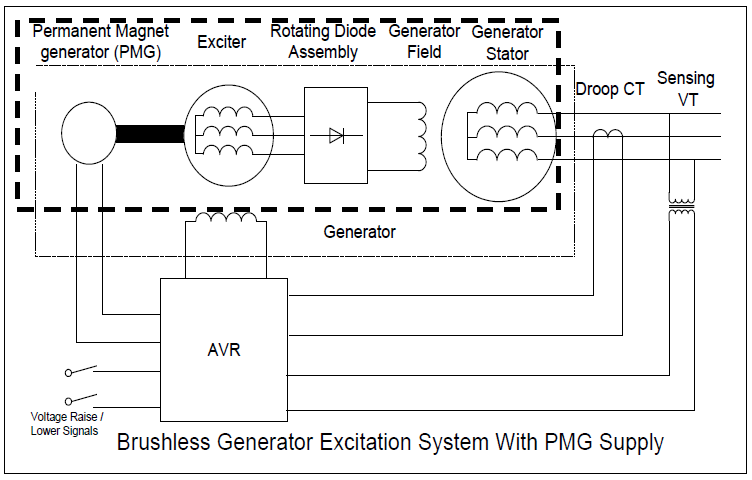
\includegraphics[width = 0.8\textwidth]{img/figure79.png}
    \caption{Brushless generator excitation system with PMG supply.}
\end{figure}
\subsection{Circuit breaker and protector initiation}
\begin{itemize}
    \item Reverse power (current)
    \item Overvoltage
    \item Significant imbalance (voltage and current)
    \item Reverse rotation
    \item Loss of excitation
    \item Negative sequence overcurrent
    \item Zero sequence overcurrent
    \item Over frequency and under frequency
    \item Thermal overloads
\end{itemize}
\section{Multi-synchronous generator operation}
\subsection{Multi-generator operation}
When generators operate in parallel to supply a power system then power may be shared between them (i.e. both \si{\kilo\watt} and \si{kVAR}). The governor and AVRs of each machine are designed to allow parallel operation. Two methods are employed:
\begin{itemize}
    \item Isochronous control: this is a modern control system which enables all generators to be controlled by computer to optimise efficiency. A computer sets the governor and AVR set points as needed by the grid.
    \item Droop control: conventional method where droop is introduced to enable sharing of \si{\kilo\watt} and \si{kVAR}
\end{itemize}
\subsection{Connection requirements}
Synchronise incoming generator with an existing system:
\begin{itemize}
    \item Same phase rotation
    \item Same frequency
    \item Same voltage level
    \item Same phase sequence
\end{itemize}
\begin{figure}[H]
    \centering
    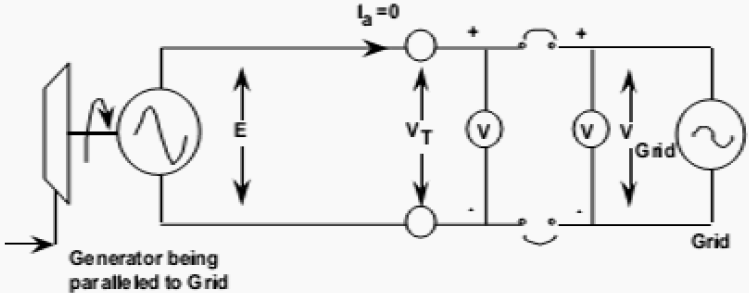
\includegraphics[width = 0.8\textwidth]{img/figure80.png}
    \caption{Synchronisation of generator to grid.}
\end{figure}
\subsection{Engine speed control}
\begin{figure}[H]
    \centering
    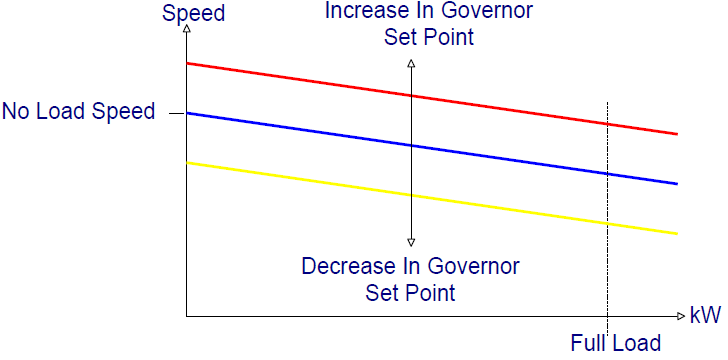
\includegraphics[width = 0.8\textwidth]{img/figure81.png}
    \caption{Single machine - governor droop characteristics (exaggerated).}
\end{figure}
\begin{itemize}
    \item Governor controls the fuel supply to a the prime mover (e.g. diesel engine or gas turbine) and forms part of a closed loop control system
    \item An increase in the governor set point gives a corresponding increase in generator speed and vice-versa
    \item Speed control system normally configured for droop control i.e. generator speed will fall as load increases
    \item \begin{gather}
              \textrm{Droop (\%)} = \frac{\textrm{No load speed} - \textrm{Full load speed}}{\textrm{No load speed}}\times 100
          \end{gather}
    \item Typical droop values 3-5\%
    \item Droop characteristic required for stable parallel operation of generators
\end{itemize}
\begin{figure}[H]
    \centering
    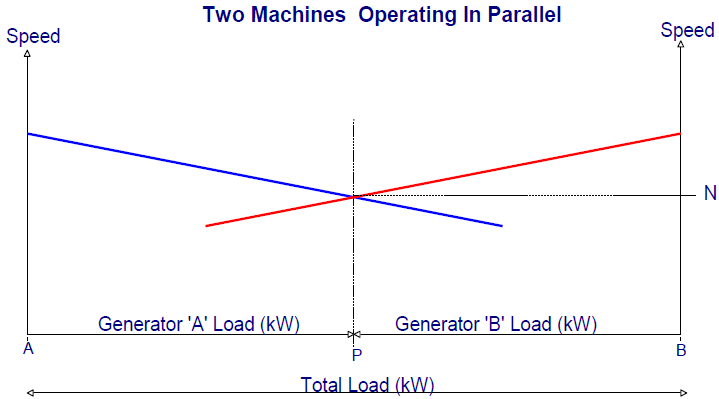
\includegraphics[width = 0.8\textwidth]{img/figure82.png}
    \caption{Two machines operating in parallel.}
\end{figure}
\begin{itemize}
    \item Fuel supply to engine determines active power supplied by the prime mover
    \item Two identical generators with the same governor droop setting will share the load equally ($PA = PB = \frac{AB}{2}$)
    \item Both machines are locked in synchronism and therefore their speeds are identical
    \item The common speed or system frequency is at the point where the two lines intersect ($N$)
\end{itemize}
\begin{figure}[H]
    \centering
    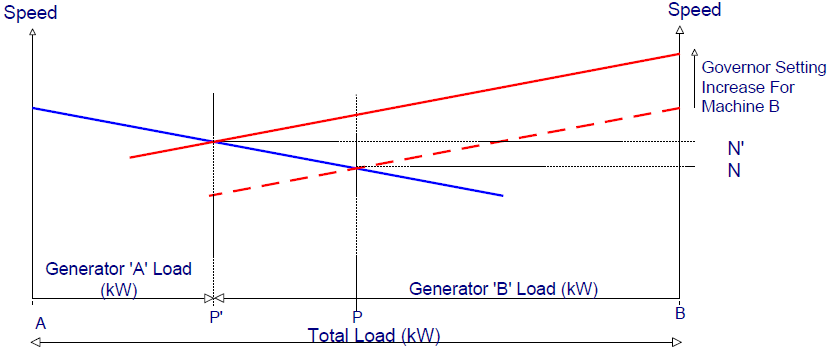
\includegraphics[width = 0.8\textwidth]{img/figure83.png}
    \caption{Two machines operating in parallel - effects due to governor adjustment.}
\end{figure}
\begin{itemize}
    \item An increase in governor setting for machine B will cause the following:
          \begin{itemize}
              \item System frequency to increase to $N'$
              \item Machine B taking a greater share of the load $BP'$
              \item Machine A taking a smaller share of the load $AP'$
          \end{itemize}
    \item System frequency may be restored back to $N$ by simultaneous reduction in both machine governor settings
\end{itemize}
\subsection{Voltage and reactive power control}
\begin{figure}[H]
    \centering
    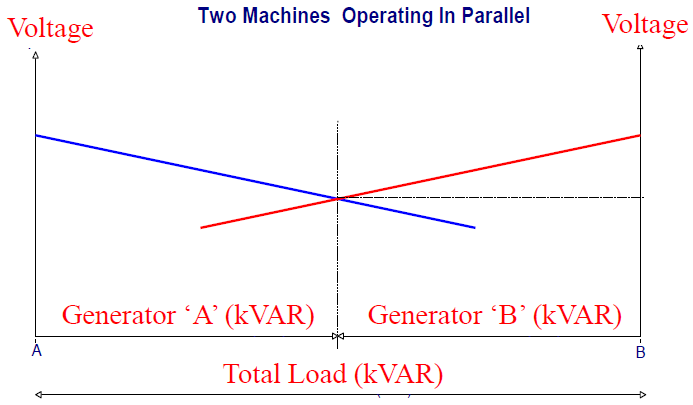
\includegraphics[width = 0.8\textwidth]{img/figure84.png}
    \caption{Two machines operating in parallel.}
\end{figure}
The AVR controls both voltage and reactive power flow. In this arrangement droop is needed (typically 1\% over the power range to ensure the two AVRs do not fight!)
\subsection{Steady state performance}
For power stations feeding a large national grid system then the voltage and frequency are stiff - this means the governor and AVR are used for controlling real and reactive power flow only. In small systems e.g. ship electrical propulsion systems, the magnitude of system load can be subject to frequency load variations and voltages and frequency is easily disturbed. Therefore, system voltage and frequency will also vary due to AVR \% governor droop respectively. Usually a Power Management Systems (PMS) is employed to supervise power system operation. PMS functionality may include the simultaneous trimming of AVR \% governor set points to maintain power system voltage and frequency to nominal, pre-set values.
\section{Generator transient performance}
\subsection{Transient performance}
Transient performance depends on the `strength of a system.' A weak system is subject to greater transient phenomena. A load transient, whether a predicted disturbance such as a motor start, or an unpredicted disturbance such as a fault at the generator busbars, will influence the power system in different ways:
\begin{itemize}
    \item Transient voltage excursions
    \item Transient frequency excursions
    \item Generator / power system instability
\end{itemize}
\begin{quoting}
    Various studies are performed at the design stage to determine the limits of power system stability taking into account both safety and operational scenarios.
\end{quoting}
\subsection{Transient load response of a generator}
\begin{figure}[H]
    \centering
    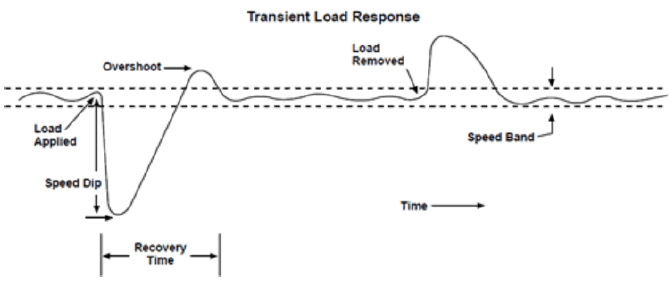
\includegraphics[width = 0.8\textwidth]{img/figure85.png}
    \caption{Transient load response of a generator.}
\end{figure}
The response to a frequency (speed) transients depends upon the governor time constants and machine characteristics.
\subsubsection{Frequency transients}
The application of an active (\si{\kilo\watt}) load will result in an increased torque and hence fuel (energy) supply requirements from the generator's prime mover. This control function is performed by the prime mover governor. Different types of prime movers react in different ways to a step load application. A lightly loaded turbo-charged diesel engine will have poor transient performance when compared to its normally aspirated equivalent.
\begin{quoting}
    The inherent voltage dip experienced on load application has the second order effect of reducing the electrical \si{\kilo\watt} load placed on the generator. This can result in improved prime mover load pick-up performance.
\end{quoting}
\subsubsection{Voltage transients}
Careful setting of the generator AVR \si{\volt}/\si{\hertz} characteristic can further improve prime mover load pick-up. If the AVR can respond by reducing generator excitation and hence generator terminal voltage when a pre set frequency level is breached, the step load change as seen by the prime mover will be reduced. The gradient of the AVR \si{\volt}/\si{\hertz} slope will also affect performance. The larger the slope, the better the load pick-up performance. However, the overall voltage dip experienced on the system will be increased.
\subsection{AVR arrangement for generator}
\begin{figure}[H]
    \centering
    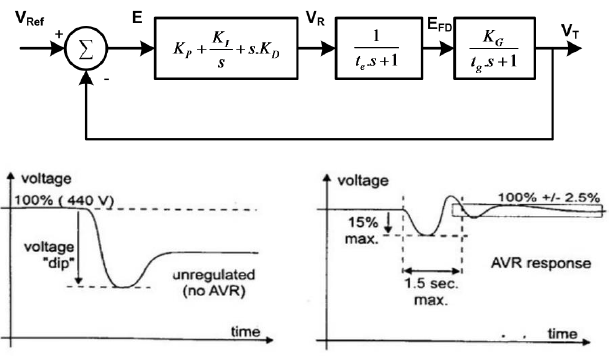
\includegraphics[width = 0.8\textwidth]{img/figure86.png}
    \caption{Typical AVR controller showing time constants for PID for exciter, regulator and field. Response must be within certain limits by regulation.}
\end{figure}
\subsubsection{Voltage transients}
A load transient will influence system voltage. The transient voltage response of the system will be dependent on the size of the load applied in relation to the generation capacity and inertia. As the generator circuit is mainly reactive, the effect on generator terminal voltage will be dependent on the power factor of the load.
\begin{quoting}
    Excessive transient voltage dips may cause connected equipment to trip on under voltage, causing a supply outage to essential pieces of equipment.
\end{quoting}
Three quantities that predominantly affect the transient performance of the generator:
\begin{itemize}
    \item Direct axis sub transient reactance $X_d''$
    \item Direct axis transient reactance $X_d'$
    \item Direct axis synchronous reactance $X_d$
\end{itemize}
For a given load application, the initial voltage dip is a function of $X_d''$ and cannot be affected by an external control system such as the generator AVR. For a constant level of excitation, generator voltage would fall to a value governed by $X_d'$ after 1 or 2 cycles. For the same level of excitation, generator voltage would eventually fall to a value consistent with $X_d$. The effects of $X_d'$ and $X_d$ can be minimised by the generator AVR supplying levels of excitation in excess to full load value (field forcing).
\begin{quoting}
    There are numerous methods and tools available in the market place to assist the engineer in determining the stability of a given power system.
\end{quoting}
\section{Generator faulted performance}
\subsection{Synchronous machine - three-phase short circuit}
\begin{figure}[H]
    \centering
    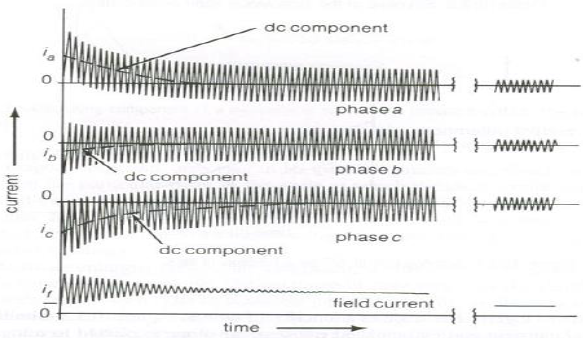
\includegraphics[width = 0.8\textwidth]{img/figure87.png}
    \caption{Typical response to a sudden three-phase short circuit at the terminals of a generator. Note the asymmetrical arrangement of the waveforms.}
\end{figure}
\subsection{Synchronous machines short-circuit envelope}
\begin{figure}[H]
    \centering
    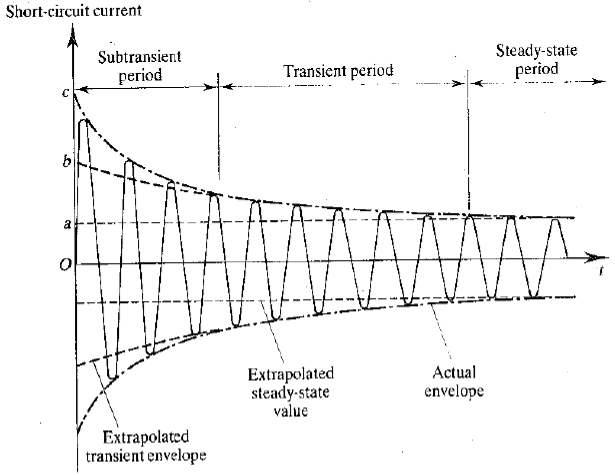
\includegraphics[width = 0.8\textwidth]{img/figure88.png}
    \caption{Synchronous machine short-circuit envelope.}
\end{figure}
\subsection{Synchronous machine short-circuit}
\begin{figure}[H]
    \centering
    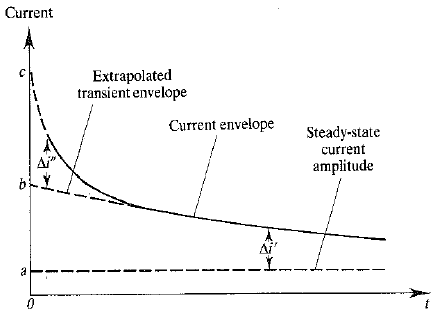
\includegraphics[width = 0.8\textwidth]{img/figure89.png}
    \caption{Synchronous machine short-circuit.}
\end{figure}
\begin{align}
    \left| I \right|   & = \frac{Oa}{\sqrt{2}} = \frac{\left|E_g\right|}{X_d}   \\
    \left| i' \right|  & = \frac{Ob}{\sqrt{2}} = \frac{\left|E_g\right|}{X_d'}  \\
    \left| i'' \right| & = \frac{Oc}{\sqrt{2}} = \frac{\left|E_g\right|}{X_d''}
\end{align}
$i''$, $X''$ and $T''$ are known as the subtransient current, subtransient reactance and subtransient time constant respectively. $i'$, $X'$ and $T'$ are known as the transient current, transient reactance and transient time constant respectively.
\subsection{Balanced three-phase component of the short-circuit current}
\begin{figure}[H]
    \centering
    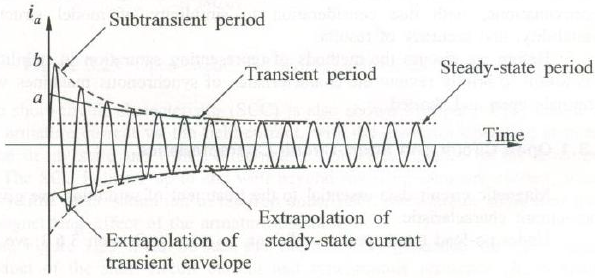
\includegraphics[width = 0.8\textwidth]{img/figure90.png}
    \caption{Balanced three-phase component of the short-circuit current.}
\end{figure}
\begin{gather}
    I = \left(\frac{E}{X_d''}-\frac{E}{X_d'}\right)e^{-\frac{t}{T_d''}} + \left(\frac{E}{X_d'}-\frac{E}{X_d}\right)E^{-\frac{t}{T_d'}}+\frac{E}{X_d}
\end{gather}
\begin{itemize}
    \item $I$: rms value of the balanced AC component
    \item $E$: rms value of the phase voltage prior to the short-circuit
    \item $t$: time after the instant of the short-circuit
    \item $X_d''$: d-axis subtransient reactance
    \item $X_d'$: d-axis transient reactance
    \item $X_d$: d-axis synchronous reactance
    \item $T_d''$: d-axis short-circuit subtransient time constant
    \item $T_d'$: d-axis short-circuit transient time constant
\end{itemize}
\subsection{Class example 1}
An \SI{11.8}{\kilo\volt} busbar is fed from three synchronous generators having the following ratings and reactances:
\begin{itemize}
    \item \SI{20}{MVA} and $X' = \SI{0.08}{pu}$
    \item \SI{60}{MVA} and $X' = \SI{0.1}{pu}$
    \item \SI{20}{MVA} and $X' = \SI{0.09}{pu}$
\end{itemize}
Calculate the fault current and MVA if a three-phase symmetrical fault occurs on the busbars using a \SI{60}{MVA} base. Explain why the transient reactance is being used instead of the subtransient for this calculation.

The transient reactance of the \SI{20}{MVA} machine has a base of $60/20 \times 0.08 = 0.24$ and $60/20 \times 0.09 = 0.27$. Hence as they are all in parallel (to a \SI{60}{MVA} base):
\begin{gather}
    Xeq = \frac{1}{\frac{1}{0.24}+ \frac{1}{0.27} + \frac{1}{0.1}} = \SI{0.056}{pu}
\end{gather}
Therefore fault MVA:
\begin{gather}
    \frac{60}{0.056} = \SI{1071}{MVA}
\end{gather}
Fault current:
\begin{gather}
    \frac{1071\times 106}{3^{0.5}\times 11800} = \SI{52402}{\ampere}
\end{gather}
\subsection{Worked example}
The per-unit reactances of a synchronous generator are $X_d =1$, $X_d' = 0.35$ and $X_d'' = 0.25$. The generator supplier a 1 per-unit load at 0.8 power factor lagging. Calculate the voltages behind the synchronous, transient and subtransient reactances. Use $V_t = 1+j0$ as base.

Since: (ignore $Ra$ as it is usually small)
\begin{gather}
    E_g = V_t + jI_LX_d
\end{gather}
Then similarly:
\begin{align}
    E_g'  & = V_t + jI_LX_d'  \\
    E_g'' & = V_t + jI_LX_d''
\end{align}
Therefore:
\begin{align}
    E_g   & = \left(1+j0\right) + j1.0  \left(0.8-j0.6\right) = \SI{1.79}{pu} \\
    E_g'  & = \left(1+j0\right) + j0.35 \left(0.8-j0.6\right) = \SI{1.24}{pu} \\
    E_g'' & = \left(1+j0\right) + j0.25 \left(0.8-j0.6\right) = \SI{1.17}{pu}
\end{align}
\subsection{Class example 2}
The system shown below is initially on no-load. Calculate the subtransient fault current that results when a three-phase fault occurs given the transformer voltage on the high side is \SI{66}{\kilo\volt}. Use vase of \SI{69}{\kilo\volt} and \SI{75}{MVA}. (Transformer = \SI{0.1}{pu} at these values).
\begin{figure}[H]
    \centering
    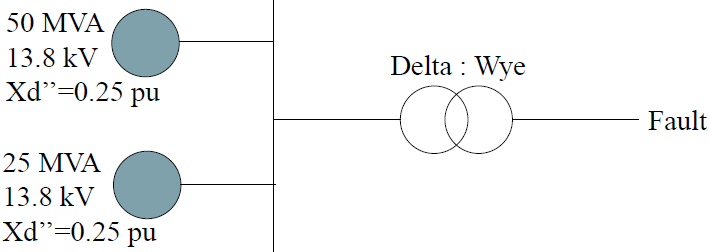
\includegraphics[width = 0.8\textwidth]{img/figure91.png}
    \caption{Class example 2 SLD.}
\end{figure}

Let the base voltage (on high side) be \SI{69}{\kilo\volt}, \SI{75}{MVA}. For G1:
\begin{gather}
    X_d'' = 0.25\times \frac{75000}{50000} = \SI{0.375}{pu}\\
    E_{g1} = \frac{66}{69} = \SI{0.957}{pu}
\end{gather}
For G2:
\begin{gather}
    X_d'' = 0.25\times \frac{75000}{25000} = \SI{0.750}{pu}\\
    E_{g2} = \SI{0.957}{pu}
\end{gather}
\begin{gather}
    X'' = \frac{0.375 \times 0.75}{0.375 + 0.75} = 0.25\\
    I'' = \frac{0.957}{j0.25 + j0.1} = -j2.735 \, \si{pu}
\end{gather}
\section{Summary}
\begin{itemize}
    \item The synchronous generator is commonly used in power systems as a stand-alone and parallel operation
    \item The synchronous machine is controller by a generator and AVR. This permits frequency and voltage to be controlled
    \item Protection of the generator is important for significant damage can occur if operated incorrectly.
    \item Transient behaviour is more significant in small networks. Fault behaviour gives rise to high fault levels and currents
\end{itemize}